% !TEX TS-program = xelatex
% !TEX encoding = UTF-8 Unicode
% WORKING!!!! File encoding: UTF-8 - file need be saved as utf8
%             Latex encoding:UTF-8 - need package utf8

\documentclass[12pt]{article}
% Margins
\usepackage[a4paper]{geometry}
\geometry{verbose,tmargin=2.5cm,bmargin=2cm,lmargin=2cm,rmargin=2cm}

%==============================================================================
% Imports
%==============================================================================
% UTF-8
\usepackage[utf8]{inputenc}
% Math formulas
\usepackage{amsmath}
% Graphics
\usepackage{graphicx} 
% Page view
\usepackage{fancyhdr}
% Matlab codes
% To use this library add mcode.sty to same folder.
% \usepackage[]{mcode}
% Subfigure caption
\usepackage{subcaption}
% Line spacing
\usepackage{setspace}
% Specific symbols (degree...)
\usepackage{gensymb}
\usepackage{titling}

%==============================================================================
% Settings
%==============================================================================
%\renewcommand{\thesection}{Úkol \arabic{section}}
\pagestyle{fancy}
\fancyhf{}
\fancyhf[HC]{\thetitle}
\fancyhf[HL,HRO]{\theauthor}
\fancyhf[HR,HLO]{\today}
\fancyhf[FL,FRO]{\thepage}
% Paragraph spacing
\setlength{\parindent}{0em}
% Line spacing
\onehalfspacing

%==============================================================================
\title{Data logger for devices connected via TCP}
\author{Albershteyn Andrey}

\date{\today}

\begin{document}

\maketitle

\section{Project structure}
%==============================================================================
% #1
%==============================================================================
\par This project is consist of two programs. First one is server which
communicate with devices by TCP-socket and process data. Parsed data from are
stored simultaneously to database and files on the disk.
\par Data can be accessed by reading files or database and also by
web-interface which is visualise data packages on the map. Internet connection
is needed to fully usage of this interface. While the map is loaded from the
third-party services. The map is also contain address and airspace information
which is also loaded from online API.

\begin{figure}[htb!]
    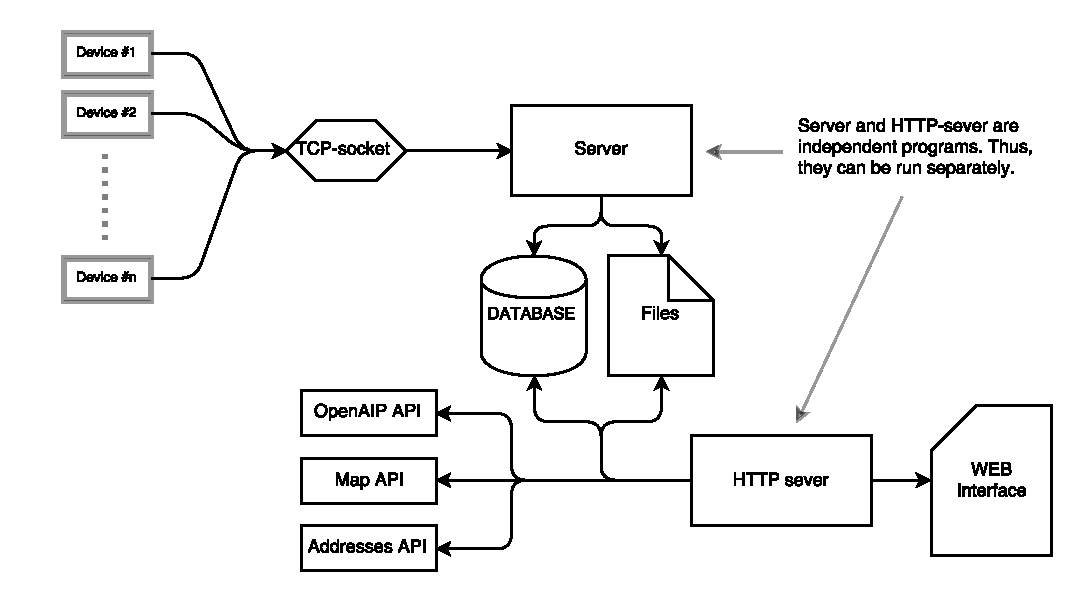
\includegraphics[width=1\textwidth]{./images/system_diagram.pdf}
    \caption{Diagram of the system and interconnection in it.}
    \label{fig:system_diagram}
    \centering
\end{figure}

\par The firgure~\ref{fig:system_diagram} shows arrangement of the system. As
can be seen there are to application "Server" and "HTTP Server". They carry
their function and don't interact with each other. Which allows us to run them
separetly. Server can be seen as a producer of the data and HTTP server is just
interface to visualise them. Data can't be changed from the HTTP server.

\begin{figure}[htb!]
    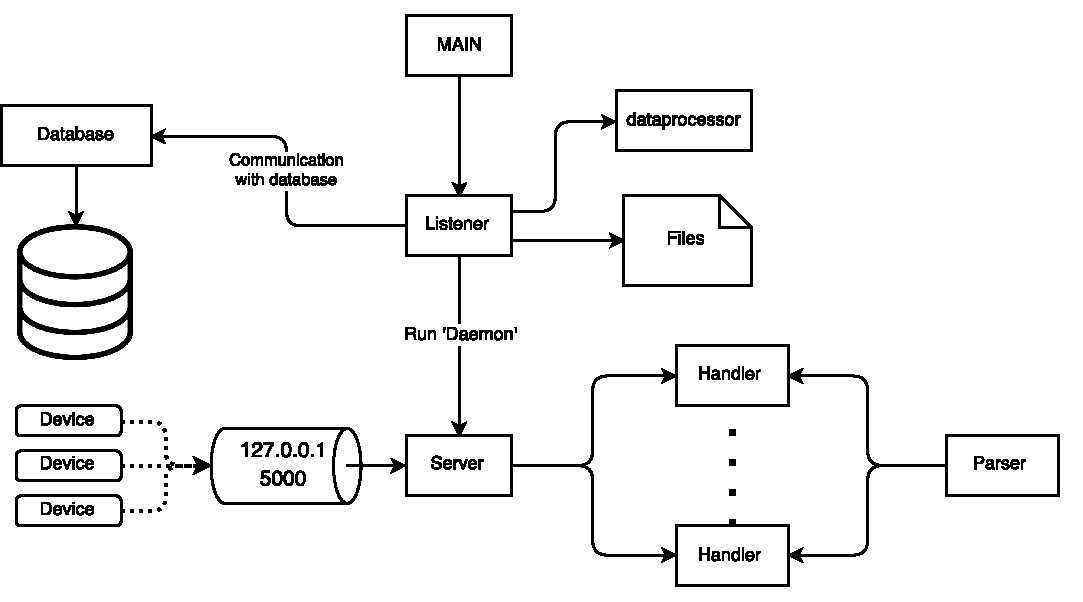
\includegraphics[width=1\textwidth]{./images/database_flow.pdf}
    \caption{Workflow of the database program.}
    \label{fig:database_flow}
    \centering
\end{figure}

\par In the figure~\ref{fig:database_flow} can be seen structure of the server
program. It is using multithreading approach to communicate with the several
deviceses at once. When device sets connection uniqe handler is created only
for this connection. If connection is closed handler is also stops.
\par Handlers parses received data from the devices. Processed data sent to
"Listener" entity which make some more changes in data (to correctly save it to
database) and than store it in the filesystem and database.

\section{Installation}
%==============================================================================
% #1
%==============================================================================
\par Ubuntu linux platform is used to test and run this software. Program is
written in Python 3 and use MySQL database for storing data. Therefore there
are several packages required to run it properly.
\par To install application on the Ubuntu machine follow next instruction:
\begin{enumerate}
    \item Download *.tar archive and put it somewhere on the targeted machine.
    \item Unpack it (using for example tar command).
    \item You will see catalog which should contain some files and source code
    of the program. 
    \item Open config.cfg and edit it as you need. This is configuration file
    for the program it will be parsed and used for installation process.
    \item After setting configuration find install.sh script. Run it.
    \item Follow the instruction shown by script installation process. You will
    be asked about installation of system packages, login information 
    for database and few other things.
    \item If there is no error messages inctallation is succesfully finished.
\end{enumerate}

\par After finishing installation there are should be new user on the target
machine. Name of this user is specified in the configuration file. Login to
this user (for example by using 'sudo username' command) and in the home
directory (/home/username) there should be catalog named as in configuration
file. 
\par TODO. Go into catalog. Run scripts for server and web-interface.

\section{Usage}
%==============================================================================
% #1
%==============================================================================
\par Data should be sent to the address of machine which runs the server with
socket port specified in the settings file.

%==============================================================================
% The bibliography 
%==============================================================================
\iffalse
\newpage
\begin{thebibliography}{1}

\bibitem{prime}
    Panos J. Antsaklis, Anthony N. Michael,
    A Linear Systems Primer,
    Birkhauser, Boston, Basel, Berlin
\end{thebibliography}
\fi

\end{document}
